\chapter{Разработка модуля анализа свойств местности, прилегающей к \ac{aes}}

\section{Модель переноса радиоактивных примесей в атмосфере} 
\label{diffusion_model}

Модель переноса радиоактивных примесей в атмосфере, которая используется при разработке проекта \ac{ascro}, основывается 
на решении полуэмперического уравнения адвекции-диффузии \cite{elokhin} методом конечных элементов. Рассмотрим это 
уравнение, описывающее перенос радиоактивной примеси в атмосфере (формула \ref{eq_diffusion}): 

\begin{equation}
    \label{eq_diffusion}
    \frac{\partial q}{\partial t} + div(\vec{U}q) + \sigma q = Dq + f
\end{equation}

с начальными условиями \ref{eq_diffusion_initials}:

\begin{equation}
	\label{eq_diffusion_initials}
    q(x, y, z, t)|_{t=0} = 0
\end{equation}

и граничными условиями \ref{eq_edges_1} --- \ref{eq_edges_3}:

\begin{equation}
	\label{eq_edges_1}
	q(x, y, z, t)|_{x=0}=0; \,\,\,\,\,\,  q(x, y, z, t)|_{y=0}=0;
\end{equation}
\begin{equation}
	\label{eq_edges_2}
	q(x, y, z, t)|_{x \rightarrow \infty}=0; \,\,\,\,\,\,  q(x, y, z, t)|_{y \rightarrow \infty}=0;
\end{equation}
\begin{equation}
	\label{eq_edges_3}
	q(x, y, z, t)|_{z \rightarrow \infty}=0; \,\,\,\,\,\, 
	k\frac{\partial q}{\partial z}|_{z=z_{0}} = (\beta - \omega)q|_{z=z_{0}}
\end{equation}

где:
\begin{description}
    \item $q$ --- концентрация радиоактивной примеси;
    \item $\vec{U}=u\vec{i} + v\vec{j} + w\vec{k}$ --- вектор скорости частиц воздуха; $\vec{i}, \vec{j}, \vec{k},$ 
    	- единичные векторы; $u, v, w$ - продольная, поперечная и вертикальная составляющие вектора скорости; 
    \item $D = \frac{\partial}{\partial x}(\mu \frac{\partial q}{\partial x}) 
    	+ \frac{\partial}{\partial y}(\mu \frac{\partial q}{\partial y})
    	+ \frac{\partial}{\partial z}(k \frac{\partial q}{\partial z})$ --- коэффициент диффузии; 
    \item $\sigma$ --- постоянная релаксации ($c^{-1}$);
    \item $\mu(x,y,z)$ --- продольно-поперечный коэффициент турбулентной диффузии;
    \item $k(x,y,z)$ --- вертикальный коэффициент турбулентной диффузии;
    \item $f$ --- источник радиоактивной примеси;
    \item $\beta$ --- скорость сухого осаждения;
    \item $\omega$ --- гравитационная скорость осаждения радиоактивной примеси;
    \item $z_{0}$ --- параметр шероховатости подстилающей поверхности.
\end{description}

\section{Необходимость анализа свойств местности}

Анализ свойств местности, прилегающей к \ac{aes}, является важной задачей при разработке модели \ac{ascro}. 

Как было показано в разделе \ref{diffusion_model}, уравнение адвекции-диффузии зависит от таких функций и параметров, 
как: скорость частиц воздуха, коэффициент диффузии, скорость сухого осаждения, скорость гравитационного осаждения и 
шероховатость подстилающей поверхности. Все перечисленные параметры явно или неявно зависят от типа местности (подробнее 
об этих параметрах описано в последующих разделах отчета), поэтому, перед построением расчетной сетки и аппроксимацией 
свойств местности на узлы расчетной сетки, необходимо разработать модуль, отвечающий за анализ свойств местности, 
прилегающей к \ac{aes}, по данным топологических карт.

\section{Принцип анализа свойств местности}

Модуль анализа свойств местности основан на обработке изображения топологической карты. При разработке модуля 
использовалась карта местности, прилегающая к Калининской \ac{aes}, расположенная вблизи города Удомля Тверской области
(рисунок \ref{fig_kalinin_map}), однако в дальнейшем модуль можно использовать для любой \ac{aes}. Масштаб карты был 
выбран таким образом, что радиус от центра карты до её верхнего края составляет порядка 30-ти километров.

Для анализа свойств местности изображение топологической карты разбивается на пиксели. Каждый пиксель изображения имеет 
свой цвет. При разработке модуля анализа свойств местности используется цветовая модель RGB. В результате разбивки 
топологической карты на пиксели получается двумерный массив, содержащий цвета пикселей в RGB-модели. 

С другой стороны, у рассматриваемой топологической карты имеется легенда, то есть таблица условных обозначений на карте 
с разъяснением их значения. По легенде карты можно понять, какой тип местности соответствует определенному цвету. Для 
примера, в таблице \ref{table_legend_map} приведена легенда карты, изображенной на рисунке \ref{fig_kalinin_map}, по 
которой можно определить интересующие нас типы местности.

В итоге, имеется двумерный массив цветов всех пикселей изображения топологической карты и легенда этой карты, 
которые можно программно сопоставить и определить, какому типу местности соответствуют каждый из пикселей. В 
дальнейшем, имея информацию о типе местности для каждого из пикселей, есть возможность спроецировать эту информацию на 
узлы расчетной сетки, разработка которой описана в последующих главах.

\begin{figure}[ht]
\centering
	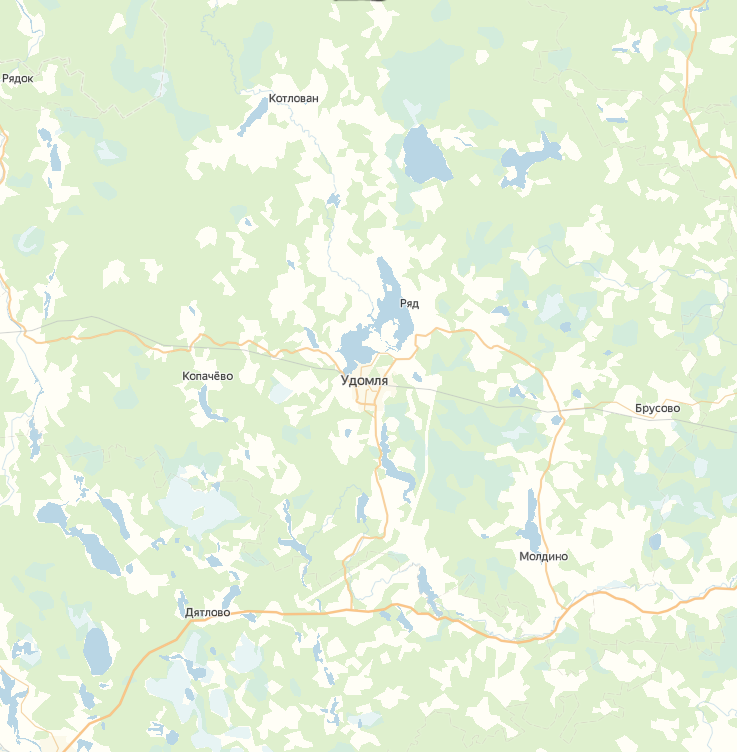
\includegraphics[width=16cm]{kalinin_test}
	\captionsetup{justification=centering}
    \caption{Топологическая карта местности, прилегающей к Калининской \ac{aes}.}
    \label{fig_kalinin_map}
\end{figure}

\begin{table}[ht]
	\setlength{\extrarowheight}{1mm}
	\caption{Соответствие типов местности на карте, изображенной на рисунке \ref{fig_kalinin_map}, и цветов в RGB-модели.}
	\label{table_legend_map}
	\centering
    \begin{tabular}{|M{0.4\textwidth}|M{0.4\textwidth}|}
    \hline Тип местности & Цвет в RGB-модели \\
    \hline Лесная местность & [212, 229, 206] \\
    \hline Водная поверхность & [170, 203, 217] \\
    \hline Городская местность & [245, 234, 197] \\
    \hline Сельскохозяйственные угодья & [255, 255, 238] \\
    \hline 
    \end{tabular}
\end{table}

\section{Разработка программного кода анализа свойств местности}

При разработке программного кода, осуществляющего анализ свойств местности, используется язык программирования Python. 

Официальный репозиторий PyPI языка Python содержит библиотеку Pillow \cite{pillow}, которая является улучшением 
библиотеки PIL (Python Imaging Library), предназначенной для работы с растровой графикой. Библиотека Pillow 
поддерживает множество форматов изображений (BMP, EPS, GIF, JPEG, PDF, PNG, PNM, TIFF и некоторых других на чтение и 
запись), позволяет преобразовывать изображения из одного формата в другой, считывать информацию об изображении, а так 
же править его. При разработке модуля анализа свойств местности используется библиотека Pillow.

Для начала, необходимо открыть файл изображения топологической карты при помощи функции \textit{open()} класса 
\textit{Image}, а затем преобразовать пиксели изображения в RGB-модель (листинг \ref{lst_image_open}):

\begin{lstlisting}[caption=Открытие изображения топологической карты, label={lst_image_open}]
from PIL import Image
img = Image.open(self.cfg.image_path)
rgb_img = img.convert("RGB")
\end{lstlisting}

Функция \textit{open()} является "ленивой" и при её вызове не происходи непосредственной загрузки изображения. Для 
загрузки информации о пикселях используется функция \textit{load()}. При вызове этой функции происходит выделение 
оперативной памяти под набор пикселей и их загрузка в память. Для более удобной работы с пикселями дополнительно 
преобразовываем их набор в \textit{numpy} массив (листинг \ref{lst_load}):

\begin{lstlisting}[caption=Загрузка информации о пикселях изображения, label={lst_load}]
img_pixels = rgb_img.load()
img_pixels_np = np.array(rgb_img)
\end{lstlisting}

Дополнительно, с помощью библиотеки Pillow, получаем такие вспомогательные параметры изображения топологической карты 
местности, как: ширина изображения в пикселях, высота изображения в пикселях, координаты центрального пикселя изображения 
и радиус изображения в пикселях (листинг \ref{lst_add_params}):

\begin{lstlisting}[caption=Получение дополнительных параметров изображения топологической карты, label={lst_add_params}]
pix_width = rgb_img.width
pix_height = rgb_img.height
img_center = [int(pix_width / 2), int(pix_height / 2)]
radius_pix = int(min([pix_width, pix_height]) / 2)
\end{lstlisting}

В итоге, на выходе модуля анализа свойств местности была получена информация о каждом пикселе изображения топологической 
карты местности, прилегающей к \ac{aes}, а так же дополнительные параметры изображения топологической карты.

\section{Заключение разработки модуля анализа свойств местности, прилегающей к \ac{aes}}

В данной главе была описана модель переноса радиоактивных примесей в атмосфере, которая используется при разработке 
проекта \ac{ascro}. Модель содержит параметры и функции, зависящие от свойств местности. С целью получения информации о 
свойствах местности, прилегающей к \ac{aes}, был разработан программный модуль, позволяющий получать эту информацию по 
данным топологических карт. В последующих главах полученная информация будет использоваться при аппроксимации свойств 
местности на узлы расчетной сетки для решения уравнения адвекции-диффузии методом конечных элементов.